\documentclass[11pt,a4paper]{article}

\usepackage{amsmath} %for mathemathic formulas
\usepackage{amssymb}
\usepackage[ngerman]{babel} %for the german language by the spellling reform (without the package the date would look like April 20, 2020)
\usepackage{enumitem} %for enumeration surrounding 
\usepackage{graphicx} %for pictures
\usepackage{siunitx}

\title{Blatt 2}
\date{\today}
\author{Hannah Rotgeri \and Feline Heinzelmann}

\begin{document}
    \maketitle

    \section*{Aufgabe 1}

    \section*{Aufgabe 2}

    \section*{Aufgabe 3}
        Elektron: \\
            Kreisumfang \(U = \SI{100}{\metre}\)
            Geschwindigkeit = \( v = 0.99*c \)
        \begin{figure}[h]
            \centering
            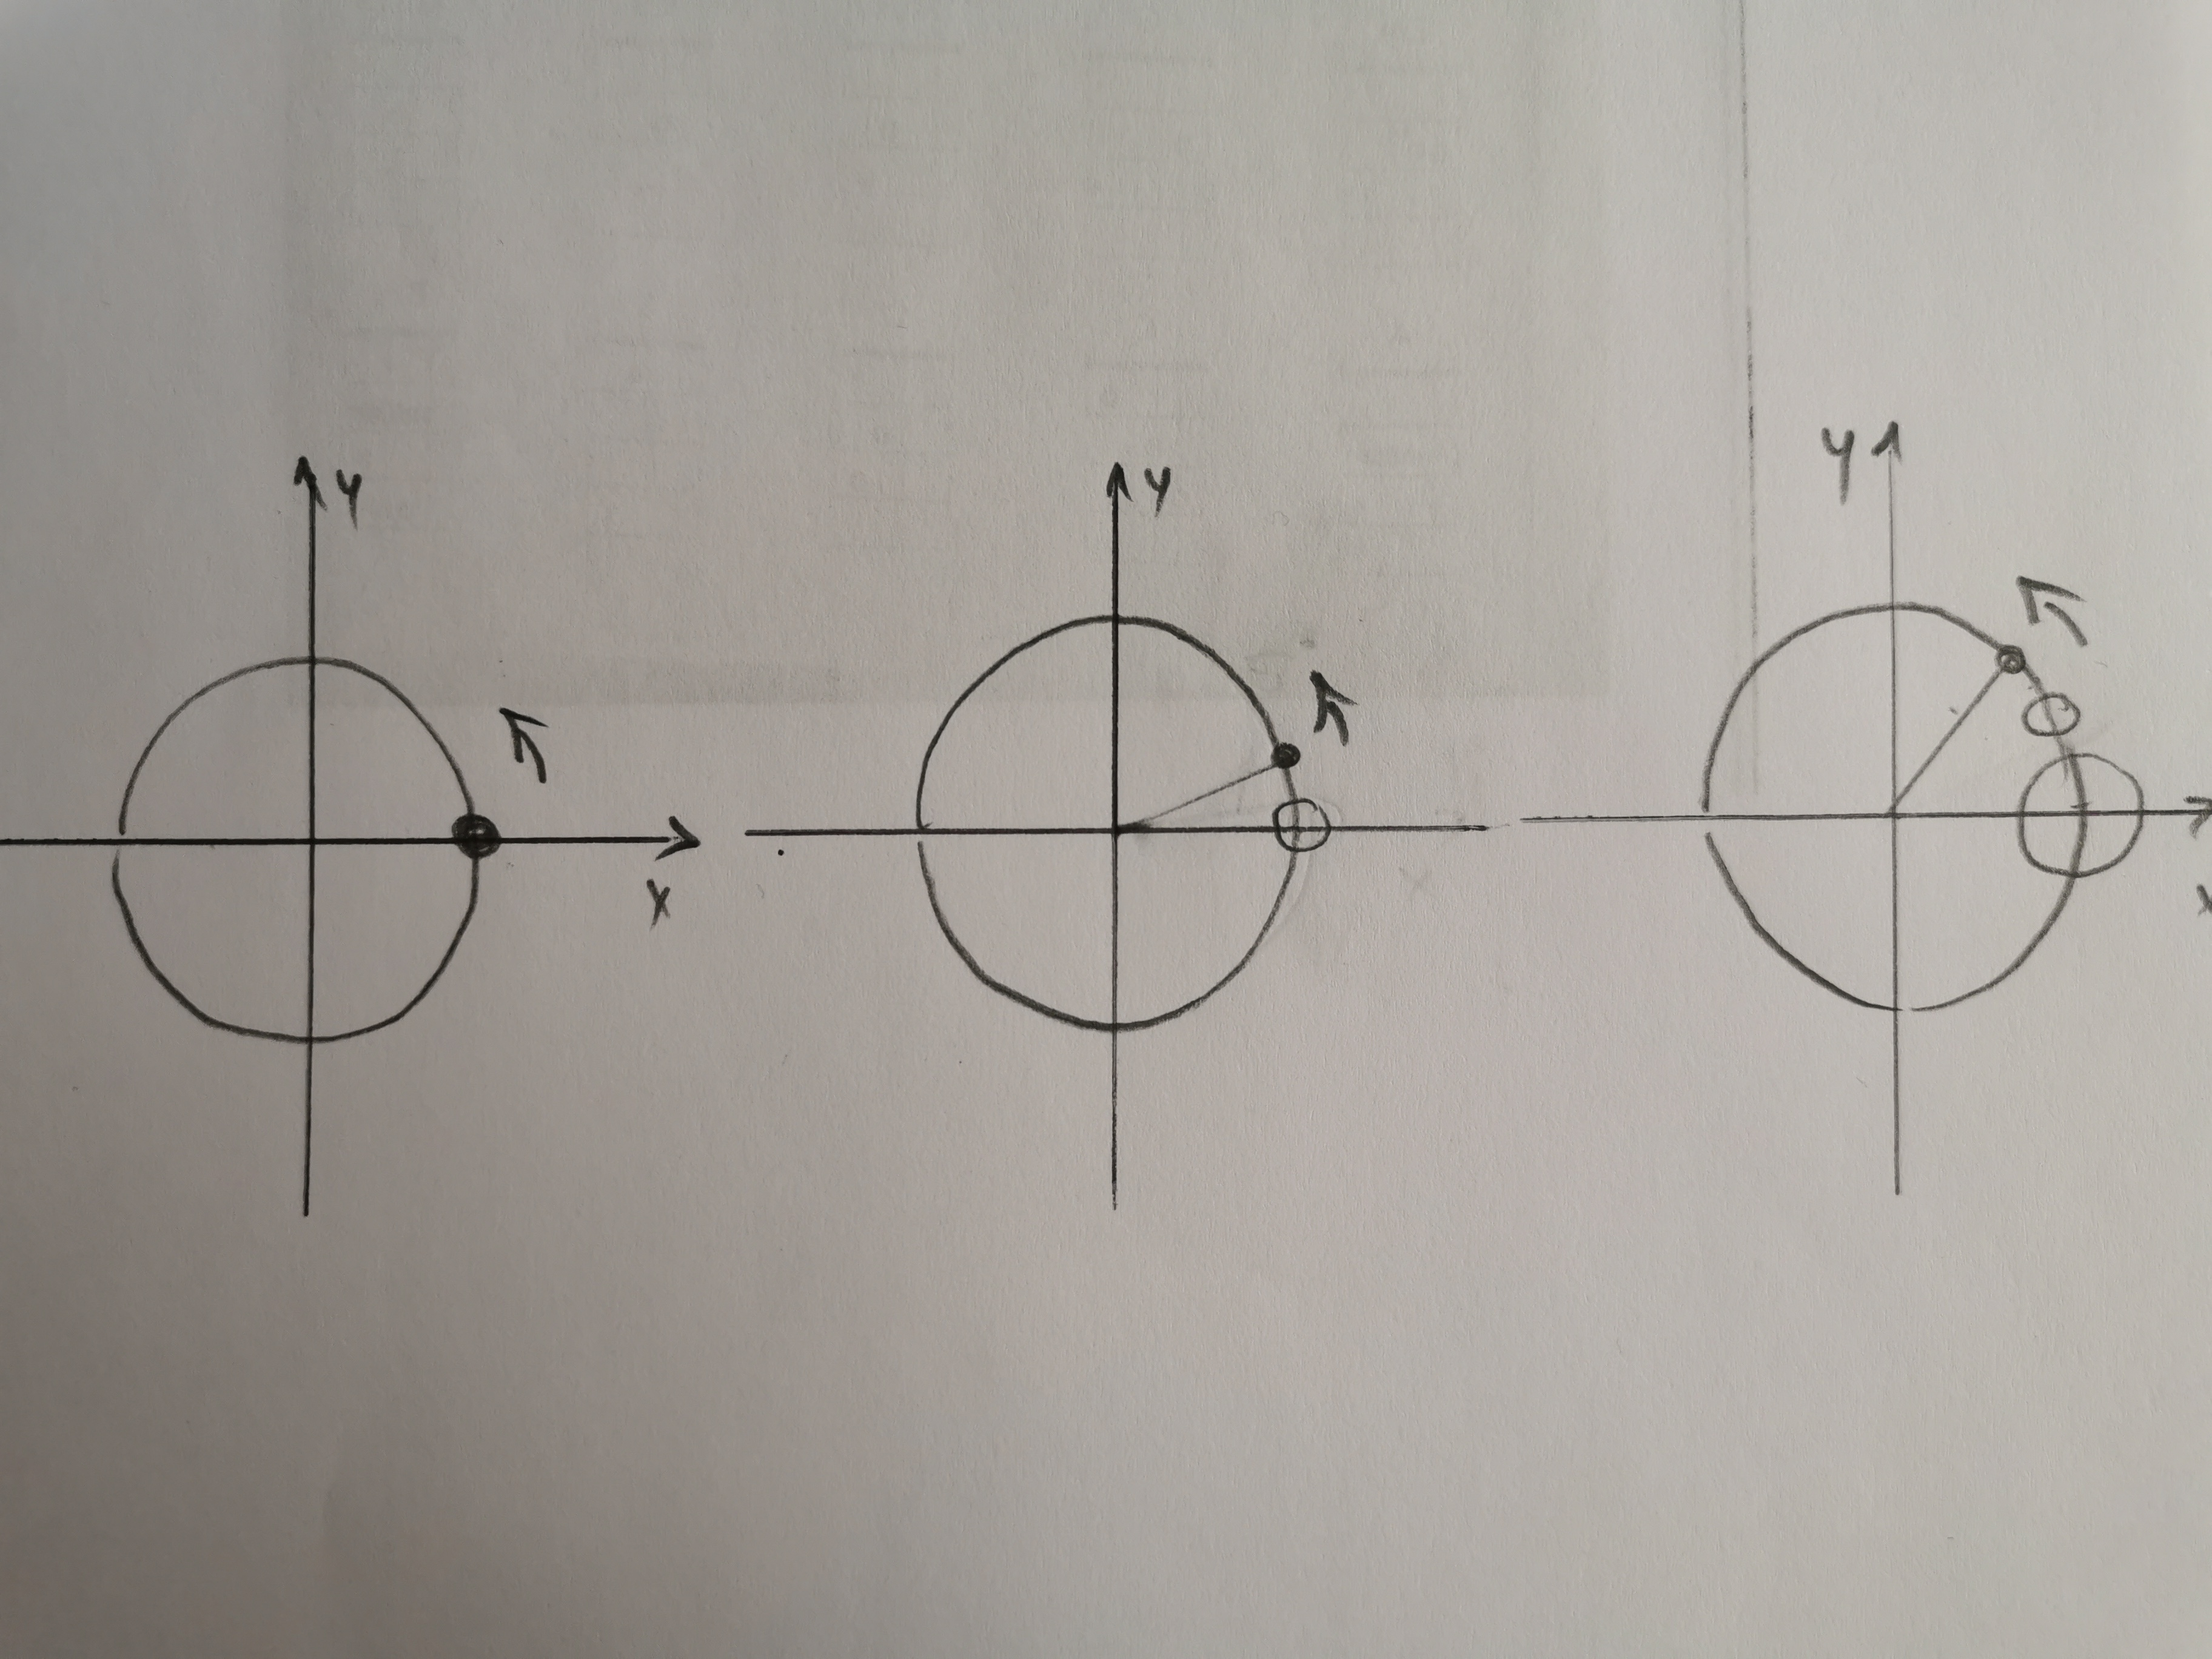
\includegraphics[width=0.7\textwidth]{Synchrotron_Skizze.jpg}
            \caption{Skizze mit der Bewegung eines Elektrons und seiner abgestrahlten Synchrotronstrahlung entlang seiner Kreisbahn}
        \end{figure}
        \begin{enumerate}
            \item Schritt: Zeit für einen Durchlauf berechnen \( t_{\mathrm{D}} = \frac{u}{v} \approx \SI{337}{\nano\second}\) 
            \item Schritt: Zeit für zwei Durchläufe berechnen, da Simulation der Synchronatronstrahlung nach zwei Runden gefragt ist \\
            \( t_{\mathrm{Stop}} = 2*t_{\mathrm{D}} \approx \SI{675}{\nano\second}\) 
            \item Schritt: Bewegung des Elektrons simulieren (Kreis)
            \item Schritt: Elektron auf Kreisbahn zu jeder Position auf dem Kreis zeichnen anhand trigonometrischer Beziehungen \\
            (\( x = r * \cos(\omega * t_{ \mathrm{aktuell} } ) , \, y = r * \sin(\omega * t_{ \mathrm{aktuell} } ) \))
            \item Schritt: Radius der Synchrotronstrahlung bestimmen \\
            \( r_{\mathrm{Syn}} = c*(t_{ \mathrm{aktuell} } - i * t_{ \mathrm{Strahlungserzeugung} } ) \) , 
            wobei i der i-te Strahlungskegel ist, der in jeweils \( 5 ^\circ\) Abständen durch das Elektron erzeugt wird; \\
            mit \( t_{\mathrm{Strahlungserzeugung}} = \frac{t_{\mathrm{D}}}{72} \) mit \( \frac{360 ^\circ}{5 ^\circ} \) 
            (Radius entspricht der Entfernung, die das Licht seit der Emission zurücklegt)
            \item Schritt: Synchrotronstrahlungskreise für zwei Umläufe zeichnen mit jeweiliger Position der Synchrotronkreise 
            nach jeweils \( 5 ^\circ\) und mit jeweiligem Radius zur betrachteten aktuellen Zeit 
        \end{enumerate}

        \begin{figure}[h]
            \centering
            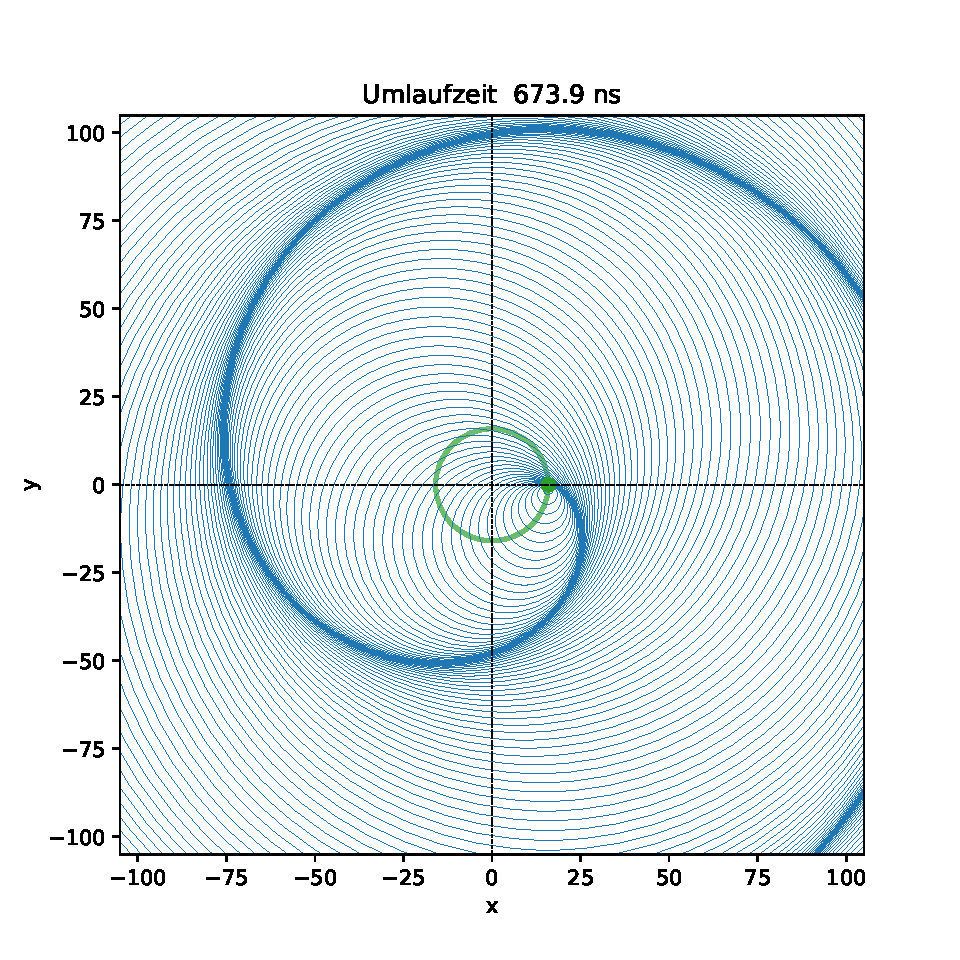
\includegraphics[width=0.7\textwidth]{synchrotron-0673.9.pdf}
            \caption{Emission von Synchrotronstrahlung nach zwei Umläufen}
        \end{figure}

        \begin{figure}[h]
            \centering
            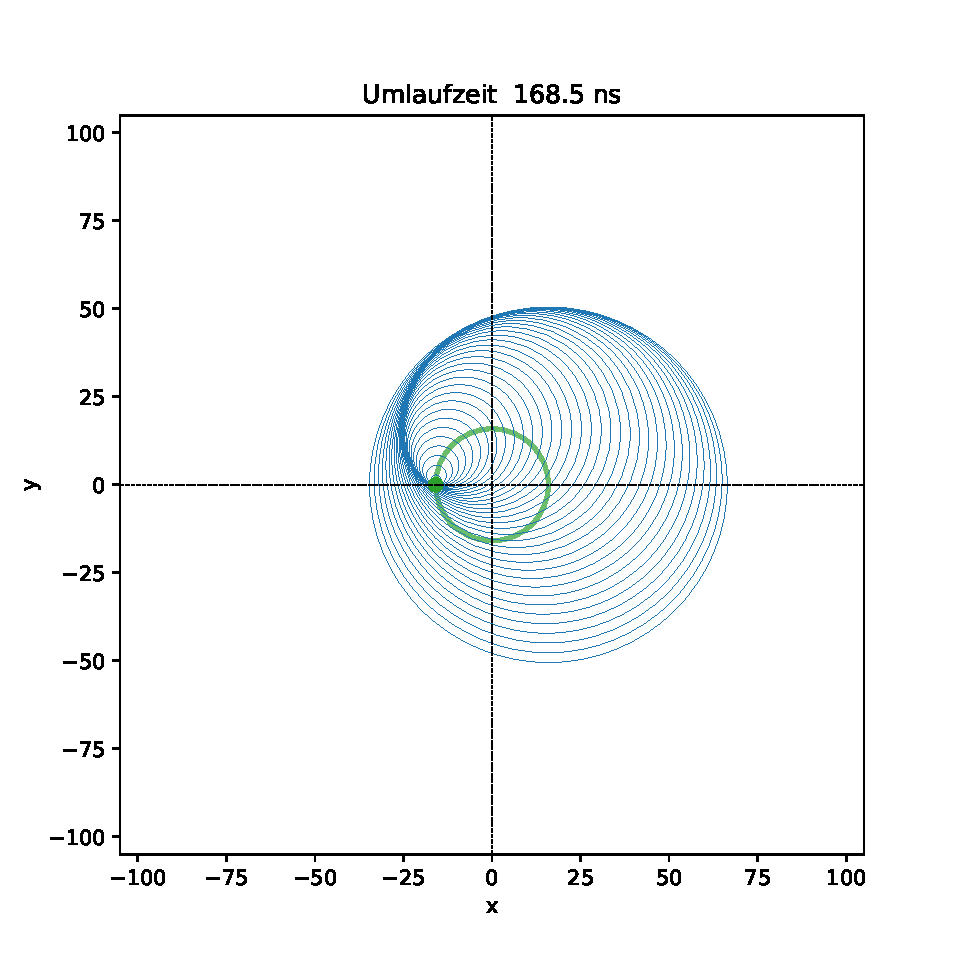
\includegraphics[width=0.7\textwidth]{synchrotron-0168.5.pdf}
        \end{figure}

        \begin{figure}[h]
            \centering
            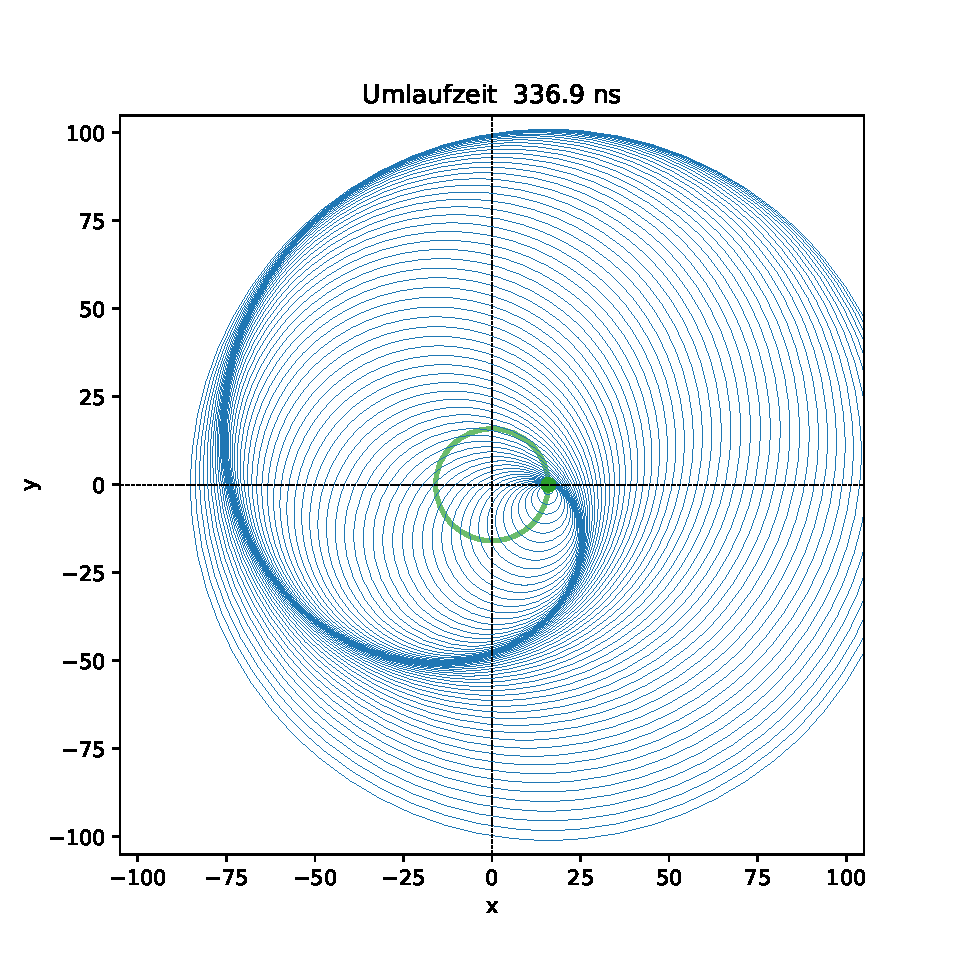
\includegraphics[width=0.7\textwidth]{synchrotron-0336.9.pdf}
        \end{figure}

\end{document}


